\section{Experiments}
\label{sec:experiments}

We randomly split the following data sets into training sets $80\%$ and
testing sets $20\%$. For multi-class data sets we do one-vs-all (OVA)
classifiers. For approximations that has reasonable run time, we will perform
cross-validation to select parameters for prior, which may have profound
impact on the result as suggested by~\cite{Asuncion2009smoothing}. 

\subsection{Data Sets}


We use 5 \href{http://archive.ics.uci.edu/ml/datasets.html}{UCI classification
datasets}:, described as in Table ~\ref{tb:datasets}.

\begin{table}
\begin{tabular}{| c | c |  c | c | c |}
  \hline
  Datasets & \# training instances & \# test instances & \# features & class-wise split\\
  \hline
  Yeast & 1500 & 917 & 103 & (14 classes) \\
  \hline
  Spambase & 3680 & 921 & 57 & 39\% vs. 61\% \\
  \hline
  Heart Diseases & 216 & 54 & 13 & 44\% vs. 56\% \\
  \hline
\end{tabular}

\caption{Datasets information}
\label{tb:datasets}
\end{table}

The Farm Ads dataset was collected from text ads found on 12 websites that 
deal with various farm animal related topics. For each ad, features include 
the words on the ad creative and the words the landing page. Words in creative 
page are diffirentiated from words from ad landing page by prefixing them with 
"ad-". Binary labels were manually added to represent if the ad is appropriate 
for that website. The Amazon Commerce reviews dataset were collected from the 
customer reviews in Amazon Commerce website for authorship identification. 
Features of a review consists of text tokens contained in that review. Labels 
represent the authors of the reviews. The dataset consists of reviews from 50 
authors, and 30 reviews per author. The p53 Mutants dataset include features 
from the biophysical models of mutant p53 proteins, and binary labels represent 
the p53 transcriptional activity (active or inactive). The Human Activity 
Recognition dataset was collected from experiments carried out with a group of 
30 volunteers. Features include acceleration and angular velocity collected from 
3 axes at constant frequency within a fixed length of time. Labels represent the 
six activities that the subjects can perform. The features of URL Reputation dataset 
include features collected for each URL, including text tokens in the URL, 
WHOIS information, location, connection speed and so on. Labels represent if 
the URL is legal. We preprocessed the datasets to evenly split multi-class 
datasets (Amazon Commerce reviews and Human Activity Recognition datasets) 
into two classes.



\footnotetext[1]{The dataset is too large so we use only one day of data out of 
total 121 days in the dataset.}

\subsection{Results}

We perform Laplace approximation, which has predictive distribution equivalent
to the MAP estimate under the same approximation. Fig.~\ref{fig:laplace} shows
that the classifier perform reasonably well on both data sets. Moreover, since
our data sets are high dimensional, it is paramount to avoid overfitting. The
classification error on test and training sets are close, demonstrating that
our prior is sufficient for these data sets. Currently we are using $\sigma =
0.05$, which is a relatively concentrated prior. As the next step we would
like to employ cross validation to select an optimal prior covariance $\sigma$.

Even though the data set is intrinsically large, fig.~\ref{fig:laplace} shows
that training on a single machine is reasonably fast. Note that training
converges in 172 and 209 iterations for p53 and farm ads data set,
respectively. Thus the run time {\em per} iteration is comparable: about $5$
seconds per iteration.


\begin{figure}[t]
\label{fig:laplace}
\centering
%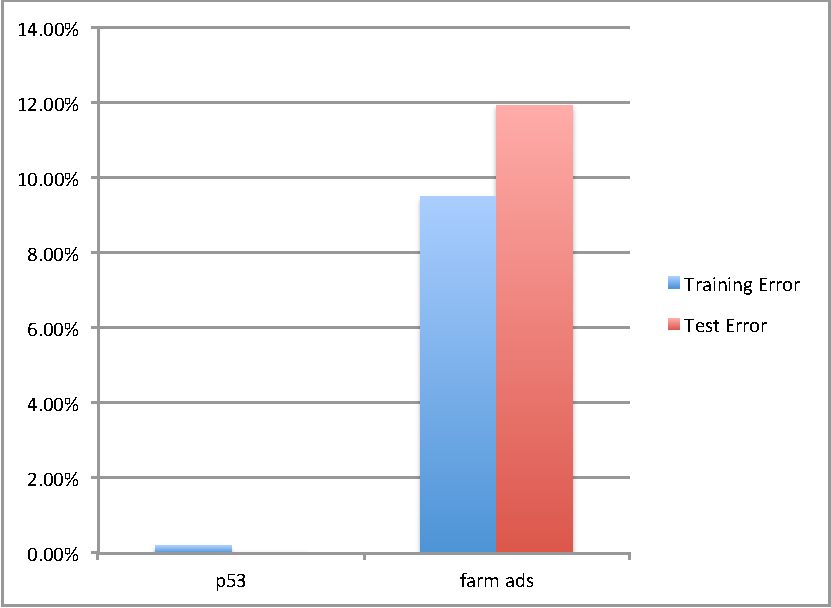
\includegraphics[height=5.0cm]{../../results/classificaiton_errors.pdf}
%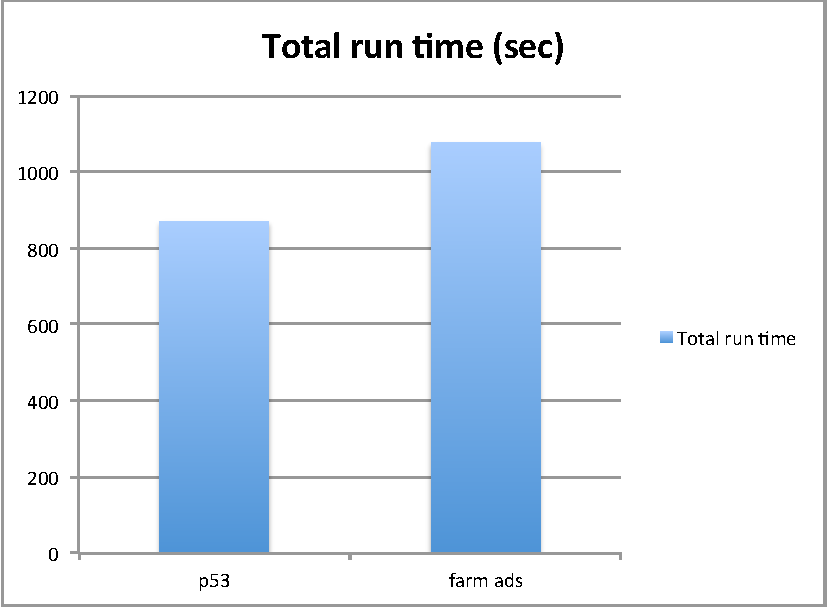
\includegraphics[height=5.0cm]{../../results/runtime.pdf}
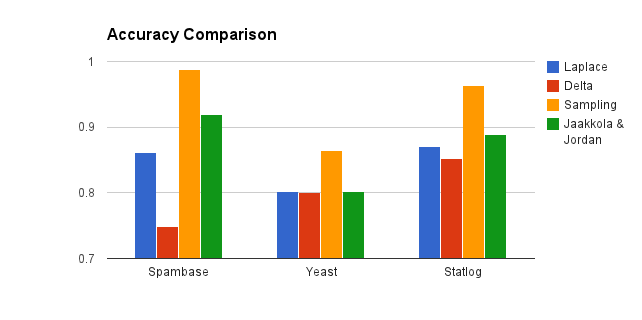
\includegraphics[height=7.0cm]{results/accuracy_comp.png}
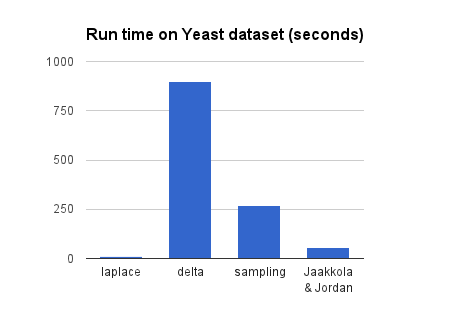
\includegraphics[height=8.0cm]{results/speed_comp.png}

\caption{\small Experiment results; {\bf Top:} Classification accuracy of all algorithms on
four datasets. {\bf Bottom:} Training time for each algorithm on Yeast dataset. }

\label{graphlab}
\end{figure}

\subsubsection{MCMC based estimation}
Our MCMC sampling strategy that we described in section~\ref{sec:MCMCmethod}
converges. Figure~\ref{fig:MCMCconverge} is a plot of the iterations of the Markov 
chain for estimation on a subset of Farms Ads dataset. This is for MLE
estimation without any priors. The X-axix of the figure represents the number of
iteration in sampling and Y-axi si the loglikelihood of theregression model We
also achieve a training accuracy of 8.57\% and a test accuracy of 9.12\% over 
this subset of datset. 

We were only able to run the experiments on this subset of the dataset as the
sampler if slow since we have a rejection sampling component besides various
other samplers. The acceptance ratio of the rejection step is is one quarter on
an average accross number of iterations. In future we plan to fins a better
alternative to this rejection sampler to achieve better speed. 

\begin{figure}[hbt]
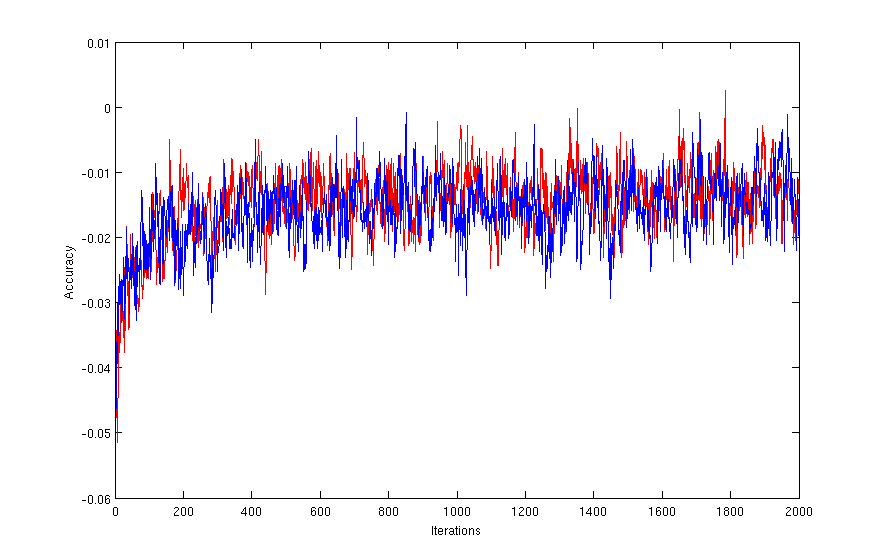
\includegraphics[width=1\textwidth]{results/KSsampleChain.png}
\caption{Two Markov chains (red and blue) converge on the same set of
parameters on the spambase dataset. The
X-axis is the number of iterations and Y-axis is the loglikelihood.}
\label{fig:MCMCconverge}
\end{figure}
